\chapter{Background}

\epigraph{
Anyone who considers arithmetical methods of producing random digits is, of course, in a state of sin.
}
% For, as has been pointed out several times, there is no such thing as a random number --- there are only methods to produce random numbers, and a strict arithmetic procedure of course is not such a method.
{\textsc{John von Neumann}}


\section{Sequential Monte Carlo}

\subsection{Motivation}
\draft{Being Bayesian. SSMs/HMMs. Example(s) of SSM (1D train?).}

\subsection{Inference in SSMs}
\draft{What quantities do we want to infer? Why is this generally difficult? Filtering, prediction, smoothing, likelihood/normalising constant.}

\subsection{Exact solutions}
\seb{This section needs redrafting, but all the content I wanted is here.}

In the case of linear Gaussian state space models, the posterior distributions of interest are also Gaussian, with mean and covariance available analytically by way of the Kalman filter \parencite{kalman1960} and Rauch-Tung-Striebel (RTS) smoother recursions \parencite{rauch1965}. Recursions are also available for some other conjugate models: see for example \textcite{vidoni1999}.
Another analytic case occurs if the state space $\mathcal{X}$ is finite, in which case any integrals become finite sums, and the forward-backward algorithm \parencite{baum1970} yields the exact posteriors.

If the model is Gaussian but non-linear, the posterior filtering distributions can be estimated using the \emph{extended Kalman filter} (see for example \textcite{jazwinski2007}), which applies a first-order linearisation in order to make use of the Kalman filter. This method performs well on models that are ``almost linear''. The resulting predictor is only \emph{optimal} when the model is actually linear, in which case the extended Kalman filter coincides with the Kalman filter.

For models that are highly non-linear or for which gradients are not readily available, a more suitable method is the \emph{unscented Kalman filter} \parencite{wan2000}. This involves taking a representative sample (which is chosen deterministically using the \emph{unscented transformation}) to characterise the distribution at time $t$, and then propagating these points through the non-linear transition $F$ to obtain a characterisation of the distribution at time $t+1$. \seb{This is getting closer to SMC, hmm?}

In more complex models such techniques are not feasible, and we are forced to resort to Monte Carlo methods.
For state space models, Markov chain Monte Carlo methods perform woefully due to the high dimension of the parameter space and high correlation between dimensions. 
But we can exploit the sequential nature of the underlying dynamics to decompose the problem into a sequence of inferences of more manageable dimension.
This is the motivation behind sequential Monte Carlo (SMC) methods.


\subsection{Feynman-Kac models}
\draft{Define a generic FK model. Show that this class includes all SSMs. Example of non-SSM that is FK?}

\subsection{Sequential Monte Carlo for Feynman-Kac models}
\draft{Present generic algorithm. State the SMC estimators of the quantities of interest. Include the dependence diagram and note that the offspring counts are not independent at each time, but can be made so by conditioning on the separatrix $\mathcal{H}$.}

\vspace{10pt}
\begin{algorithm}
\DontPrintSemicolon
\KwData{$N, T, \mu, (K_t)_{t=1}^T, (g_t)_{t=0}^T$}
\lFor{$i \in \{1,\dots,N\}$}{ 
	Sample $X_0^{(i)} \sim \mu(\cdot)$
}
\lFor{$i \in \{1,\dots, N\}$}{
		$w_{0}^{(i)} \gets  \left\{{\sum_{j=1}^N g_0(X_0^{(j)})}\right\}^{-1}{g_0(X_0^{(i)})} $ 
	}
\For{$t \in \{0,\dots, T-1\}$}{
	Sample $a_t^{(1:N)} \sim $ \textsc{resample}$(\{1,\dots ,N\}, w_t^{(1:N)}$)\;
	\lFor{$i \in \{1,\dots,N\}$}{
		Sample $X_{t+1}^{(i)} \sim K_{t+1}(X_t^{(a_t^{(i)})}, \cdot)$
	}
	\lFor{$i \in \{1,\dots, N\}$}{	
		$w_{t+1}^{(i)} \gets \Big\{ {\sum_{j=1}^Ng_{t+1}(X_t^{(a_t^{(j)})},X_{t+1}^{(j)}) }\Big\}^{-1} g_{t+1}(X_t^{(a_t^{(i)})},X_{t+1}^{(i)}) $
	}
}
\caption{Sequential Monte Carlo}\label{alg:SMC}
\end{algorithm}
\vspace{10pt}

Figure \ref{fig:cond_indep_graph} shows part of the conditional dependence graph implied by Algorithm \ref{alg:SMC}. Our aim is to find a $\sigma$-algebra $\mathcal{H}_t$ at each time $t$ that separates the ancestral process (encoded by $a_t^{(1:N)}$) from the filtration $\mathcal{F}_{t-1}$. That is, $a_t^{(1:N)}$ is conditionally independent of $\mathcal{F}_{t-1}$ given $\mathcal{H}_t$.
By a D-separation argument \parencite[see][]{verma1988}, the nodes highlighted in grey suffice as the generator of $\mathcal{H}_t$. That is, for each $t$, we take
\begin{equation*}
\mathcal{H}_t = \sigma(X_{t-1}^{(1:N)}, X_t^{(1:N)}, w_{t-1}^{(1:N)}, w_t^{(1:N)} ).
\end{equation*}
Notice that $\nu_t^{(1:N)}$ can be expressed as a function of $a_t^{(1:N)}$, and as such carries less information.
\begin{figure}[h]
\centering
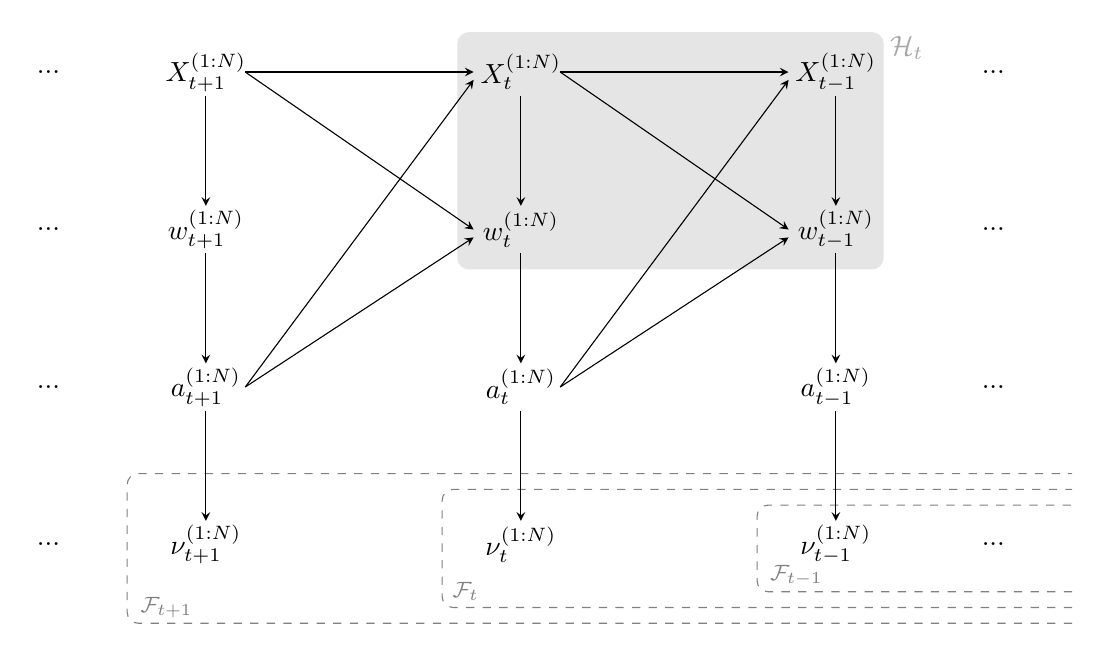
\begin{tikzpicture}[>=stealth]
% separatrix
\filldraw[gray!20, rounded corners] (3.2,0.5)--(8.6,0.5)--(8.6,-2.5)--(3.2,-2.5)--cycle;
\node[gray!70] at (8.9,0.3) {$\mathcal{H}_t$};
% left dots
\node at (-2,0) {...};
\node at (-2,-2) {...};
\node at (-2,-4) {...};
\node at (-2,-6) {...};
% labels (t+1)
\node at (0,0) {$X_{t+1}^{(1:N)}$};
\node at (0,-2) {$w_{t+1}^{(1:N)}$};
\node at (0,-4) {$a_{t+1}^{(1:N)}$};
\node at (0,-6) {$\nu_{t+1}^{(1:N)}$};
% labels t
\node at (4,0) {$X_{t}^{(1:N)}$};
\node at (4,-2) {$w_{t}^{(1:N)}$};
\node at (4,-4) {$a_{t}^{(1:N)}$};
\node at (4,-6) {$\nu_{t}^{(1:N)}$};
% labels (t-1)
\node at (8,0) {$X_{t-1}^{(1:N)}$};
\node at (8,-2) {$w_{t-1}^{(1:N)}$};
\node at (8,-4) {$a_{t-1}^{(1:N)}$};
\node at (8,-6) {$\nu_{t-1}^{(1:N)}$};
% right dots
\node at (10,0) {...};
\node at (10,-2) {...};
\node at (10,-4) {...};
\node at (10,-6) {...};
%filtrations
\draw [rounded corners, dashed, gray] (11,-6.6)--(7,-6.6)--(7,-5.5)--(11,-5.5);
\draw [rounded corners, dashed, gray] (11,-6.8)--(3,-6.8)--(3,-5.3)--(11,-5.3);
\draw [rounded corners, dashed, gray] (11,-7)--(-1,-7)--(-1,-5.1)--(11,-5.1);
% filtration labels
\node[gray] at (7.5,-6.4) {\footnotesize{$\mathcal{F}_{t-1}$}};
\node[gray] at (3.3,-6.6) {\footnotesize{$\mathcal{F}_{t}$}};
\node[gray] at (-0.5,-6.8) {\footnotesize{$\mathcal{F}_{t+1}$}};
% arrows (t+1) -> t
\draw[->] (0.5,0)--(3.4,0);
\draw[->] (0.5,0)--(3.4,-2);
\draw[->] (0.5,-4)--(3.4,-2.1);
\draw[->] (0.5,-4)--(3.4,-0.1);
% arrows t -> (t-1)
\draw[->] (4.5,0)--(7.4,0);
\draw[->] (4.5,0)--(7.4,-2);
\draw[->] (4.5,-4)--(7.4,-2.1);
\draw[->] (4.5,-4)--(7.4,-0.1);
% vertical arrows (t+1)
\draw[->] (0,-0.3)--(0,-1.7);
\draw[->] (0,-2.3)--(0,-3.7);
\draw[->] (0,-4.3)--(0,-5.7);
% vertical arrows t
\draw[->] (4,-0.3)--(4,-1.7);
\draw[->] (4,-2.3)--(4,-3.7);
\draw[->] (4,-4.3)--(4,-5.7);
% vertical arrows (t-1)
\draw[->] (8,-0.3)--(8,-1.7);
\draw[->] (8,-2.3)--(8,-3.7);
\draw[->] (8,-4.3)--(8,-5.7);
\end{tikzpicture}
\caption[Conditional dependence structure of SMC algorithm]{Part of the conditional dependence graph implied by Algorithm \ref{alg:SMC}. The direction of time is from left to right. The reverse-time filtration is indicated by the dashed areas. The nodes highlighted in grey generate the separatrix $\mathcal{H}_t$ between $a_t^{(1:N)}$ and $\mathcal{F}_{t-1}$.\seb{Use the same shades of grey here as elsewhere}}
\label{fig:cond_indep_graph}
\end{figure}


\subsection{Theoretical justification}
\draft{How come SMC works? Convergence results (briefly!) e.g. Lp bounds, CLT, stability.}


\section{Coalescent theory}

\subsection{Kingman's coalescent}
\draft{Define the $n$-coalescent, and Kingman's coalescent as extension of it. (Do I need to introduce random partitions first?)}
\seb{Include Kingman citations!}
\begin{defn}
\label{def:kingman}
The \emph{$n$-coalescent} is the homogeneous continuous-time Markov process on the set of partitions of $\{1,\dots,n\}$ with infinitesimal generator $Q$ having entries
\begin{equation}\label{eq:KCgenerator}
q_{\xi,\eta} = \begin{cases}
1 & \xi \prec \eta\\
-|\xi|(|\xi|-1)/2 & \xi=\eta \\
0 & \text{otherwise}
\end{cases}
\end{equation}
where $\xi$ and $\eta$ are partitions of $\{1,...,n\}$, $|\xi|$ denotes the number of blocks in $\xi$, and $\xi \prec \eta$ means that $\eta$ is obtained from $\xi$ by merging exactly one pair of blocks.
\end{defn}
The $n$-coalescent can also be characterised as the restriction to $[n]$ of \emph{Kingman's coalescent}, the analogous process supported on partitions of $\mathbb{N}$.
Kingman's coalescent is a canonical model in coalescent theory, underpinned by the rich theory of exchangeable random partitions. An excursion into these areas is beyond the scope of this work, since our results only ever consider finite samples from the population (the setting of the $n$-coalescent), but an excellent introduction to Kingman's coalescent from this perspective can be found in \textcite[Chapters 1--2]{berestycki2009}. \seb{or \textcite{wakeley2009} ?}

\begin{figure}
\centering
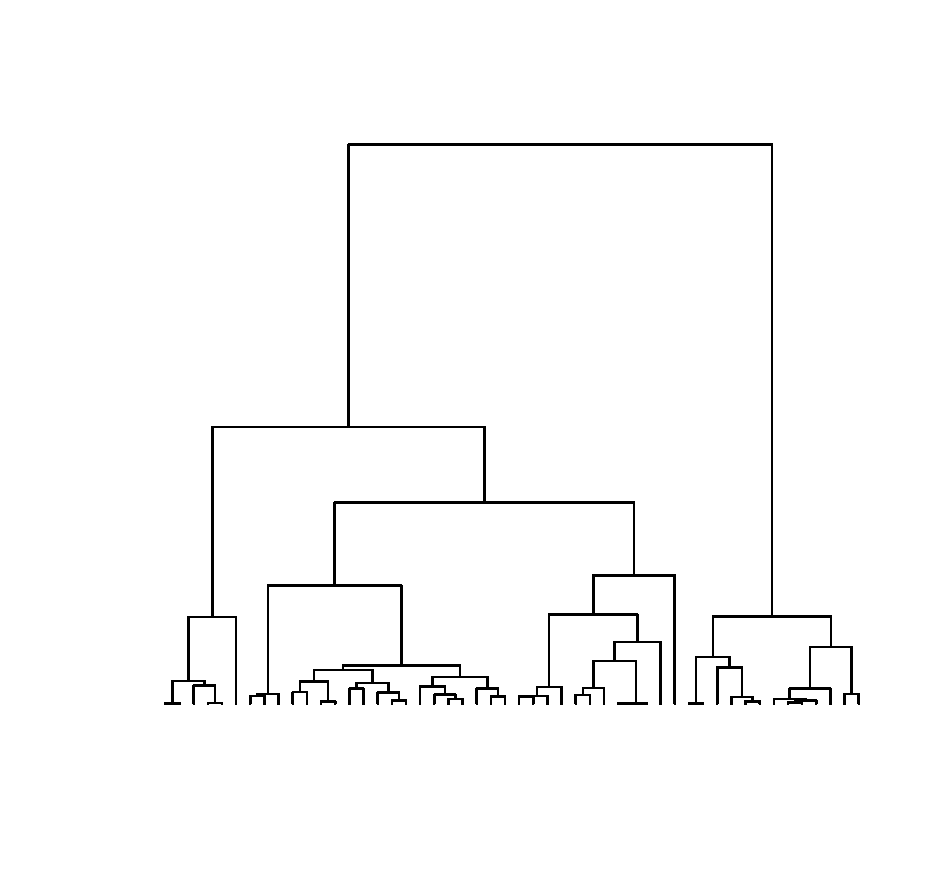
\includegraphics[width=0.6\textwidth, trim={2.8cm 3cm 1.5cm 2cm}, clip]{plots/ncoalescent.pdf}
\caption[The $n$-coalescent]{A realisation of the $n$-coalescent with $n=50$.}
\end{figure}


\subsection{Properties}
\draft{Properties of Kingman's coalescent / $n$-coalescent. Distributions of branch length, waiting times, time to MRCA. Coming down from infinity.}

The simplicity of $Q$ allows various properties of the $n$-coalescent to be studied analytically.
Starting with $n$ blocks, exactly $n-1$ coalescences are required to reach the absorbing state where all blocks have coalesced, known in the population genetics literature as the \emph{most recent common ancestor} (MRCA).

\seb{Include a diagram clarifying definitions of $t_i, T_i, T_{MRCA}$; similar to the KC realisation but smaller $n$ and all the relevant time intervals labelled.}
Denote by $t_2, t_3 \dots, t_n$ the waiting times between coalescent events, where $t_i$ is the amount of time for which the coalescent has exactly $i$ distinct lineages.
A simple consequence of Definition~\ref{def:kingman} is that these waiting times are independent and have distributions
\begin{equation}
t_i \sim \Exp\left( \binom{i}{2} \right) .
\end{equation}
%The waiting times between coalescence events $t_1, t_2, \dots, t_{n-1}$ \seb{it would probably be better to define $t_k=$ time spent with $k$ lineages, to make indexing less confusing} are independent and distributed according to
%\begin{equation}
%t_i \sim \Exp\left( \binom{n-i+1}{2} \right) .
%\end{equation}
The partial sum $T_k := \sum_{i=k+1}^n t_i$ gives the total time up to the $(n-k)^{th}$ coalescence event, i.e.\ the first time at which there are only $k$ lineages remaining. 
%This has the distribution
%\begin{equation}
%T_{MRCA} 
%\eqdist \sum_{i=1}^{n-1} \Exp\left( \binom{n-i+1}{2} \right)
%\end{equation}
%under which many expectations can be calculated explicitly.
Of particular interest is the time to the most recent common ancestor, $T_{MRCA} := T_1$.
With some algebra we find, for instance,
\begin{align}
\E[ T_{MRCA} ] 
= \sum_{i=2}^{n} \E[t_i]
= \sum_{i=2}^n \frac{2}{i(i-1)}
= 2 \sum_{i=2}^n \left\{ \frac{1}{i-1} - \frac{1}{i} \right\}
= 2 \left( 1 - \frac{1}{n} \right) .
%\underset{n\to\infty}{\longrightarrow} 2 .
\end{align}
and
\begin{equation}
\V[ T_{MRCA} ] 
= \sum_{i=2}^n \V[t_i]
= \sum_{i=2}^n \left( \frac{2}{i(i-1)} \right)^2
\underset{n\to\infty}{\longrightarrow} \frac{4}{3}(\pi^2 - 9) .
\end{equation}
\seb{Plot mean with sd-ribbon over $n$ for an illustration?}\\
\seb{We are not taking $n\to\infty$ so why are these limits of interest?? Perhaps an approximation would be more useful (like harmonic numbers $\simeq$ log thing).}
Another quantity of interest is the total branch length,
$ L := \sum_{i=2}^n i t_i $.
For instance
\begin{equation}
\E[ L ] 
= \sum_{i=2}^n i \E[ t_i ]
= \sum_{i=2}^n \frac{2}{i-1}
= \sum_{i=1}^{n-1} \frac{2}{i} ,
\end{equation}
a harmonic series, and
\begin{equation}
\V[ L ] 
= \sum_{i=2}^n i^2 \V[ t_i ]
= \sum_{i=2}^n \frac{4}{(i-1)^2}
= \sum_{i=1}^{n-1} \frac{4}{i^2} .
\end{equation}


\subsection{Models in population genetics}
The Kingman coalescent is the limiting coalescent process (in the large population limit) for a surprisingly wide range of population models. Some important examples of models in Kingman's ``domain of attraction'' are introduced in this section.
Common to all of these models are the following assumptions:
\begin{itemize}
\item The population has constant size $N$
\item Reproduction happens in discrete generations
\item The offspring distributions are identical at each generation, and independent between generations
\item These models are all \emph{neutral}, i.e.\ the offspring distribution is exchangeable.
\end{itemize}
\seb{Since offspring exchangeable, distribution of parental indices equivalent to distribution of offspring counts. Define offspring counts in terms of parental indices. Explain what ``neutral'' means from the biological perspective.}

\subsubsection{Wright-Fisher model}
The neutral Wright-Fisher model \parencite{fisher1923, fisher1930, wright1931} is one of the most studied models in population genetics.
At each time step the existing generation dies and is replaced by $N$ offspring. The offspring descend from parents $(a_1, \dots, a_N)$ which are selected according to
\begin{equation*}
a_i \overset{iid}{\sim} \Cat(\{1, \dots, N\}, (1/N, \dots, 1/N)).
\end{equation*}
The joint distribution of the offspring counts is therefore
\begin{equation*}
(v_1,\dots, v_N) \sim \Mn(N, (1/N, \dots, 1/N)).
\end{equation*}
Since the Multinomial distribution is exchangeable, this model is neutral.
There are several non-neutral variants of the Wright-Fisher model \seb{citations?}, but they are typically much less tractable than the neutral one.

Kingman showed in his original papers introducing the Kingman coalescent \parencite{kingman1982gene} that, under a certain time-scaling, genealogies of the neutral Wright-Fisher model converge to the Kingman coalescent as $N\to\infty$.

\subsubsection{Cannings model}
The neutral Cannings model \parencite{cannings1974, cannings1975} is a more general construction which encompasses the neutral Wright-Fisher model as a special case.

In the Cannings model, the particular offspring distribution is not specified; we only require that it is exchangeable, i.i.d.\ between generations, and preserves the population size. In particular, the probability of observing offspring counts $(v_1, \dots, v_N)$ must be invariant under permutations of this vector.

Genealogies of the neutral Cannings model also converge to the Kingman coalescent, under some conditions and a suitable time-scaling, as $N\to\infty$ \parencite[Section 2.2]{etheridge2011}.

\subsubsection{Moran model}
The neutral Moran model \parencite{moran1958}, while perhaps less biologically relevant, is mathematically appealing because its simple dynamics make it particularly tractable.

At each time step, an ordered pair of individuals is selected uniformly at random. The first individual in this pair dies (i.e.\ leaves no offspring in the next generation), while the other reproduces (leaving two offspring). All of the other individuals leave exactly one offspring.
%Usually the model is thought of as having ``overlapping generations'': the individuals having one offspring are considered to be not reproducing but rather surviving to appear again in the next generation.
%However, one can equally think of it as having non-overlapping generations and a low variance reproduction mechanism.
This is another special case of the neutral Cannings model, where the offspring distribution is now uniform over all permutations of $(0,2,1,1,\dots,1)$.
Therefore we know that under a suitable time-scaling, its genealogies converge to the Kingman coalescent.
\seb{Something should be said about the difference between Moran and WF time scales at this point.}

%The mathematical tractability of this model stems from the fact that, if we formulate it a little more carefully, its pre-limiting behaviour is exactly that of a rescaled Kingman coalescent. This requires us to work in continuous time, and now we say that the pairs are chosen to die/reproduce with exponential rate $\binom{N}{2}$. This gives the unit pairwise merger rate we need, and we can clearly see that the only possible mergers are between one pair of lineages at a time.


\subsection{Particle populations}
\draft{Particles = individuals, iterations = generations. In what ways is SMC like a population model? (constant population size, non-overlapping generations, discrete time). In what ways is SMC not like a population model? (non-neutral, non-Markov?)}


\section{Sequential Monte Carlo genealogies}

\subsection{From particles to genealogies}
\draft{How does the SMC algorithm induce a genealogy? (resampling = parent-child relationship).}

\subsection{Performance}
\draft{How do genealogies affect performance? Variance (and variance estimation?), storage cost. Ancestral degeneracy.}

\subsection{Mitigating ancestral degeneracy}
\draft{Low-variance resampling (save details for next section). Adaptive resampling: idea of balancing weight/ancestral degeneracy; rule of thumb for implementing it; when is it effective or not?; necessary changes to our generic SMC algorithm (calculation of weights in particular). Backward sampling: when is it possible to do this?}

\subsection{Asymptotics}
\draft{Why are large population asymptotics useful? Existing results (path storage, KJJS).}


\section{Resampling}

\subsection{Definition}
\draft{The job of resampling (map weights to counts). Define ``valid'' resampling schemes (the three rules). Counter-examples where these rules are violated (the examples I've mentioned in previous writings, plus optimal transport resampling [see email from James Thornton] and that one FC told me about recently [Huang et al 2020]).}

\subsection{What makes a good resampling scheme?}
\draft{Low-variance: variance of what? Different criteria/ definitions of optimality. Negative association. Link back to adaptive resampling: interaction between adaptive and low-variance resampling.}

\subsection{Examples}
\draft{Tour of the key resampling schemes (multinomial, residual-*, stratified, systematic, and the worst possible scheme). Comparison of properties of these, existing results comparing schemes. Implementation considerations. Theoretical justification (or lack of).}

\subsection{Stochastic rounding}
\draft{Define stochastic rounding. Resampling schemes contained by this class. General properties for this class (marginal distributions, negative association, minimum-variance).}


\section{Conditional SMC}

\subsection{Particle MCMC}
\draft{Motivate particle MCMC methods.}

The idea behind particle MCMC methods is to use SMC steps within the MCMC updates in a way that improves the mixing properties of the Markov chain.
In certain models, generally those including some highly correlated sequential components, this strategy can be very effective.

The following scenario illustrates the power of particle MCMC, and is a good model to have in mind as we go on to discuss particle Gibbs and ancestor sampling.
\draft{Include the model from the start of my ancestor sampling note. Emphasise that the inference itself is not sequential; we are targeting one static posterior distribution, on a fixed time horizon.}


\subsection{Particle Gibbs algorithm}
\draft{Present particle Gibbs algorithm (for the specific model just introduced?, but note that of course the algorithm is more general). Explain why CSMC is required within particle Gibbs.}

\subsection{Ancestor sampling}
\draft{Algorithm (or required changes to generic algorithm). Relation to backward sampling. When can it be implemented? Effect on performance (when is it effective?). Maybe illustrate/motivate with some plots as in the ancestor sampling note.}
